\section*{Introduction}

NeuraNet is a C library providing structures and functions to implement a neural network.\\ 

The neural network implemented in NeuraNet consists of a layer of input values, a layer of output values, a layer of hidden values, a set of generic base functions and a set of links. Each base function has 3 parameters (detailed below) and each links has 3 parameters: the base function index and the indices of input and output values. A NeuraNet is defined by the parameters' values of its generic base functions and links, and the number of input, output and hidden values.\\

The evaluation of the NeuraNet consists of taking each link, ordered on index of values, and apply the generic base function on the first value and store the result in the second value. If several links has the same second value index, the sum value of all these links is used. However if several links have same input and output values, the outputs of these links are multiplied instead of added (before being eventually added to other links having same output value but different input value).\\

The generic base functions is a linear function. However by using several links with same input and output values it is possible to simulate any polynomial function. Also, there is no concept of layer inside hidden values, but the input value index is constrained to be lower than the output one. So, the links can be arranged to form layers of subset of hidden values, while still allowing any other type of arrangement inside hidden values. Also, a link can be inactivated by setting its base function index to -1. Finally, the parameters of the base function are constrained to [-1.0,1.0].\\

NeuraNet provides functions to easily use the library GenAlg to search the values of base functions and links' parameters. An example is given in the unit tests (see below). It also provides functions to save and load the neural network (in JSON format).\\

NeuraNet has been validated on the Iris data set.\\

It uses the \begin{ttfamily}PBErr\end{ttfamily} library.\\

\section{Definitions}

The generic base function is defined as follow:\\
\begin{equation}
B(x)=\left[tan(1.57079*b_0)(x+b_1)+b_2\right]\cap[-1.0,1.0]
\end{equation}
where $\left\lbrace b_0,b_1,b_2\right\rbrace\in[-1.0,1.0]^3$ are the parameters of the base function and $x\in\mathbb{R}$ and $B(x)\in\mathbb{R}$.

\section{Interface}

\begin{scriptsize}
\begin{ttfamily}
\verbatiminput{/home/bayashi/Coding/NeuraNet/neuranet.h}
\end{ttfamily}
\end{scriptsize}

\section{Code}

\subsection{pbmath.c}

\begin{scriptsize}
\begin{ttfamily}
\verbatiminput{/home/bayashi/Coding/NeuraNet/neuranet.c}
\end{ttfamily}
\end{scriptsize}

\subsection{pbmath-inline.c}

\begin{scriptsize}
\begin{ttfamily}
\verbatiminput{/home/bayashi/Coding/NeuraNet/neuranet-inline.c}
\end{ttfamily}
\end{scriptsize}

\section{Makefile}

\begin{scriptsize}
\begin{ttfamily}
\verbatiminput{/home/bayashi/Coding/NeuraNet/Makefile}
\end{ttfamily}
\end{scriptsize}

\section{Unit tests}

\begin{scriptsize}
\begin{ttfamily}
\verbatiminput{/home/bayashi/Coding/NeuraNet/main.c}
\end{ttfamily}
\end{scriptsize}

\section{Unit tests output}

\begin{scriptsize}
\begin{ttfamily}
\verbatiminput{/home/bayashi/Coding/NeuraNet/unitTestRef.txt}
\end{ttfamily}
\end{scriptsize}

neuranet.txt:\\
\begin{scriptsize}
\begin{ttfamily}
\verbatiminput{/home/bayashi/Coding/NeuraNet/neuranet.txt}
\end{ttfamily}
\end{scriptsize}

bestnn.txt:\\
\begin{scriptsize}
\begin{ttfamily}
\verbatiminput{/home/bayashi/Coding/NeuraNet/bestnn.txt}
\end{ttfamily}
\end{scriptsize}
\iffalse
\begin{center}
\begin{figure}[H]
\centering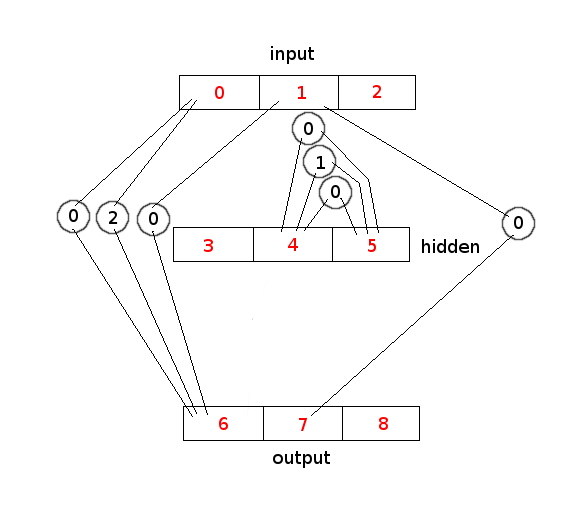
\includegraphics[width=10cm]{./example.png}\\
\end{figure}
\end{center}

Bases:\\

\begin{tabular}{cc}
id&B(x)\\
0&$tan(0.504549*1.57079)*(x-0.819784)+0.832003=1.014387x+0.000414$\\
1&$tan(-0.313292*1.57079)*(x+0.050474)-0.576482=-0.536109x-0.603541$\\
2&$tan(-0.519646*1.57079)*(x+0.646151)+0.701341=-1.063698x+0.01403$\\
\end{tabular}\\

Values:\\

\begin{tabular}{cc}
id&value\\
0&x\\
1&y\\
2&z\\
6& $(-1.079001x^2+0.01379x+1.014387y+0.000419)/2$ (target: $(-x^2+y)/2$)\\
7& $1.014387y+0.000414$ (target: $y$)\\
8& 0 (target: 0)\\
\end{tabular}
\fi
\section{Validation}

\subsection{Iris data set}

Source: https://archive.ics.uci.edu/ml/datasets/iris \\

main.c:\\
\begin{scriptsize}
\begin{ttfamily}
\verbatiminput{/home/bayashi/Coding/NeuraNet/Examples/Iris/main.c}
\end{ttfamily}
\end{scriptsize}

learning:\\
\begin{scriptsize}
\begin{ttfamily}
\verbatiminput{/home/bayashi/Coding/NeuraNet/Examples/Iris/learn.txt}
\end{ttfamily}
\end{scriptsize}

validation:\\
\begin{scriptsize}
\begin{ttfamily}
\verbatiminput{/home/bayashi/Coding/NeuraNet/Examples/Iris/check.txt}
\end{ttfamily}
\end{scriptsize}
